
\section{Hardware setup and event data\label{sec:Hardware-setup-and}}

This section describes the hardware setup and gives an intuition of
the event data that a DVS produces.


\subsection{DVS and its interface\label{sec:interface}}

The DVS has a standard USB 2.0 interface. The sensor is distributed
with a portable software framework written in Java called jAER~\cite{jaer}.
For this project we used C++ for maximum efficiency. So we developed
a special driver to be developed, based on the Thesycon USB device
driver~\cite{thesycon}. The events are transmitted from the sensor
in packets of up to several hundred events; however, each event is
still independently tagged at the source with its proper timestamp.



\subsection{Active LED Markers (\ALMs)\label{sec:leds}}

We used infrared LEDs since the DVS is most sensitive in the infrared
spectrum.  The LED controller is based on the Bronze Board~\cite{bronzeboard}
from inilabs, which is based on an AVR32.  The controller drives
the LEDs using PWM.



In our setup we could easily change the PWM frequency to the LEDs.
An upper bound on the detectable frequency depends on the power of
the LEDs and the distance to the sensor. A DVS is not magic: there
must be a large enough change in the number of photons reaching the
photoreceptor to trigger an event. In our setup we found 2~KHz to
be an adequate value as an upper bound. The frequencies for each LEDs
were then decided in the interval 1--2~KHz making sure we did not
choose frequencies with common harmonics. A reasonable lower bound
on the blinking frequency was found experimentally to be $1$~KHz,
so that those frequencies would not be confused with the events triggered
by the background motion.


\subsection{Statistical properties of event sequences}

\prettyref{fig:events-hist} gives an intuition of how the stream
of events looks like. In this scenario both the \ALMs and the DVS
are fixed. \prettyref{fig:events-hist}\emph{a} shows the histogram
of the number of events coming from a particular pixels. The three
peaks are three \ALMs at frequencies $f=500,700,1000\,\mbox{Hz}$.
The number of events is different for each peak because the frequencies
differ. The halo in \prettyref{fig:events-hist}\emph{a} cannot be
explained by the refractive properties of the optics, and is probably
due to non-ideal local interactions among neighbors in the sensing
array.

\prettyref{fig:events-hist}\emph{b} shows the sequence of events
obtained from one particular pixel, corresponding to the \ALM  with
a frequency of 1~KHz. There is a different number of~\pP and~\pN
events. This implies that it is not possible to interpret these events
as the derivative of the image.

For this particular data, the~\pP events arrive noisily, while the~\pN
events arrive more regularly. Note that the what we observe here is
the combination of the LED dynamics with the dynamics of the photoreceptor
and the nonlinear detector. Experimentally, we found that the interval
between successive \pP/\pN transitions is repeatable. For this data,
the jitter is well approximated by a Gaussian with standard deviation
equal to $6$~$\mu$s (\prettyref{fig:events-hist}\emph{c}).


\subsection{Effects of sensor motion\label{sub:Alternate-events-and-motion}}

If the sensor is moving, events are generated from the apparent motion
of the environment as well as the \ALMs. However, we have found that
we can discriminate between the two types of events based on their
temporal statistics. 

\prettyref{fig:switch-hist} shows the histogram of frequencies of
the \pP/\pN transitions in three scenarios: a)~a stationary camera
looking at stationary \ALMs; b)~a moving camera looking at stationary
\ALMs; c)~a moving camera with no LEDs. From this data we can see
that the sensor motion generates a large number of events and transitions,
but the corresponding frequencies are low ($<600$~Hz in this case),
so that we can still clearly see the peaks originated from the \ALMs-generated
events. Therefore, by choosing the blinking frequencies high enough,
it is possible to filter out the sensor motion just by ignoring the
events corresponding to frequencies under a certain threshold. 

\vfill

\begin{figure}[H]
\centering{}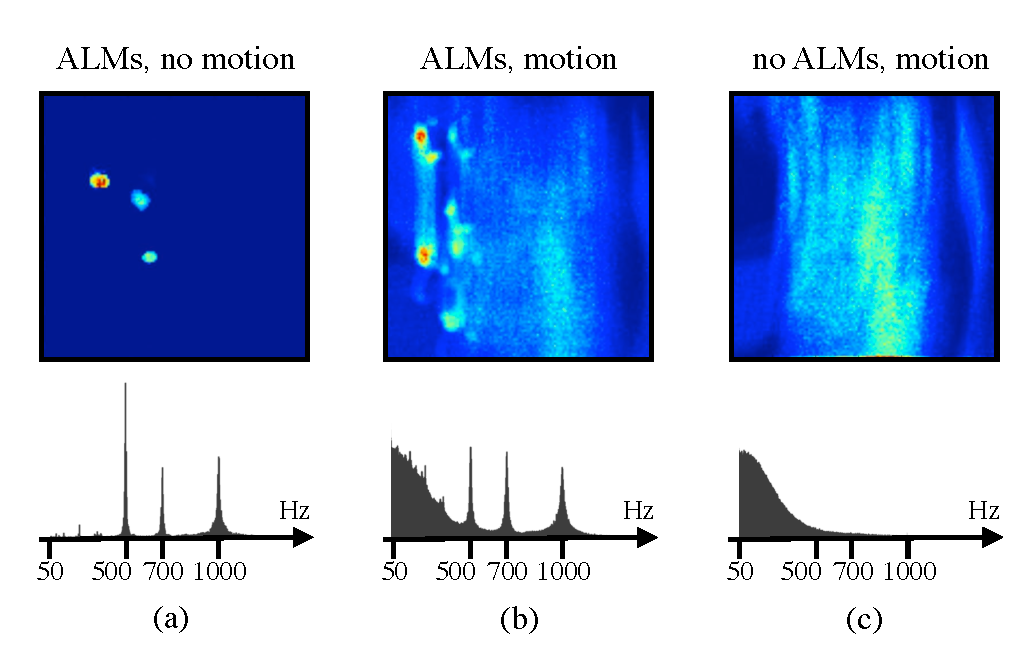
\includegraphics[bb=15bp 5bp 483bp 300bp,clip,width=8.6cm]{figures/slides/motion_small}\caption{\label{fig:switch-hist}This figure shows the statistics of the intervals
between \pP/\pN transitions, in three different scenarios. The upper
row shows the number of events generated by each pixel over in an
interval of a few seconds. The bottom row shows the histograms of
the inverse of the interval between successive \pP/\pN transitions
at each pixel. (a)~In the first case, both \ALMs and sensor are
stationary. The observed frequencies correspond to the three \ALMs.
(b)~In the second case, the sensor is moving with respect to the
\ALMs and the environment. (c)~In the third case the sensor is moving
and the \ALMs have been switched off. In (b)~and~(c) the motion
of the camera creates apparent motion of the environment which generates
a large number of events and transitions. However, those transitions
have low frequency. In this case, the events generated from the background
motion are negligible after $700$~Hz, though this depends on the
statistics of the environment and the speed of the motion. We can
choose the frequencies of the markers high enough such that they are
not confused with the background motion.}
\end{figure}

